\documentclass{beamercours}
\title{Cours TalENS 2023-2024}
\subtitle{RRrrr, Shadoks, Craies}
\author{Matthieu Boyer}
\definecolor{mint}{HTML}{9ffeb0}

\begin{document}
\maketitle
\begin{frame}{Plan}\tableofcontents[sectionstyle=show]
\end{frame}
\section*{Introduction}
\begin{frame}
    \frametitle{\tt Lights Out !}
    \begin{figure}
        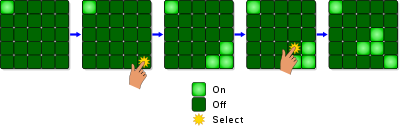
\includegraphics[scale = .5]{Fichiers/lights-out.png}
        \caption{Déroulé d'une partie de \texttt{Lights Out}}
    \end{figure}
    Source : \href{https://upload.wikimedia.org/wikipedia/commons/thumb/a/a9/LightsOutIllustration.svg/400px-LightsOutIllustration.svg.png}{Wikipédia}\\
    \visible<2>{Il existe aussi des variantes du jeu où les lumières peuvent avoir plus que deux couleurs possibles}

\end{frame}

\section{Modélisation}
\begin{frame}
    \frametitle{État du Jeu}
    On part par exemple d'une situation semblable à celle-ci dessous :
    \begin{center}
        \vspace{-17pt}
        \begin{tikzpicture}
            \foreach \i in {0,...,2}{
                    \foreach \j in {0, ..., 2}{
                            \draw[black, double, fill = mint] (\i, \j) rectangle +(1, 1);
                        }
                }
            \draw[decorate, decoration = {calligraphic brace}] (0.1, 3.1) -- node[above] {$m$} (2.9, 3.1) ;
            \draw[decorate, decoration = {calligraphic brace}] (-0.1, 0.1) -- node[left] {$n$} (-0.1, 2.9) ;
            \draw[fill = vulm] (2.01, .01) rectangle +(.98, .98);
            \draw[fill = vulm] (.01, 2.01) rectangle +(.98, .98);
            \draw[fill = vulm] (2.01, 2.01) rectangle +(.98, .98);
            \draw[fill = vulm] (1.01, 1.01) rectangle +(0.98, 0.98);
            \draw[fill = vulm] (2.01, 1.01) rectangle +(0.98, 0.98);
            \draw[fill = yulm] (1.01, .01) rectangle +(0.98, 0.98);

            \draw[black, double, fill = vulm] (3.5, 1) rectangle +(1, 1);
            \draw[black, double, fill = yulm] (5.5, 1) rectangle +(1, 1);
            \draw[black, double, fill = mint] (7.5, 1) rectangle +(1, 1);
            \draw[black, double, fill = vulm] (9.5, 1) rectangle +(1, 1);
            \draw[black, ->] (4.55, 1.5) -- (5.45, 1.5);
            \draw[black, ->] (6.55, 1.5) -- (7.45, 1.5);
            \draw[black, ->] (8.55, 1.5) -- (9.45, 1.5);
        \end{tikzpicture}
    \end{center}
    \only<2>{On choisit de modéliser chaque couleur par un nombre différent : Violet = 0, Jaune = 1 et Menthe = 2}
    \only<3>{On décrit alors la situation par la couleur de chaque lumière sous forme d'un vecteur : \vspace{-12pt}
        \[\mP = \left(0, 2, 0, 2, 0, 0, 2, 1, 0\right)\vspace{-12pt}\]
        La lumière de la case $i, j$ est représenté par la $i * m + j$-ème valeur.}
\end{frame}

\begin{frame}
    \frametitle{Transitions de l'État du Jeu - 1}
    Si on appuie sur la lumière en haut au milieu :
    \begin{center}
        \begin{tikzpicture}
            \foreach \i in {0,...,2}{
                    \foreach \j in {0, ..., 2}{
                            \draw[black, double, fill = mint] (\i, \j) rectangle +(1, 1);
                        }
                }
            \draw[fill = vulm] (2.01, .01) rectangle +(.98, .98);
            \draw[fill = vulm] (.01, 2.01) rectangle +(.98, .98);
            \draw[fill = vulm] (2.01, 2.01) rectangle +(.98, .98);
            \draw[fill = vulm] (1.01, 1.01) rectangle +(0.98, 0.98);
            \draw[fill = vulm] (2.01, 1.01) rectangle +(0.98, 0.98);
            \draw[fill = yulm] (1.01, .01) rectangle +(0.98, 0.98);

            \draw[black, ->] (3.05, 1.5) -- node[above]{$L_{0, 1}$} (3.95, 1.5);

            \foreach \i in {4,...,6}{
                    \foreach \j in {0, ..., 2}{
                            \draw[black, double, fill = mint] (\i, \j) rectangle +(1, 1);
                        }
                }

            \draw[fill = yulm] (4.01, 2.01) rectangle +(.98, .98);
            \draw[fill = vulm] (5.01, 2.01) rectangle + (.98, .98);
            \draw[fill = yulm] (6.01, 2.01) rectangle +(.98, .98);
            \draw[fill = mint] (4.01, 1.01) rectangle +(0.98, 0.98);
            \draw[fill = yulm] (5.01, 1.01) rectangle +(0.98, 0.98);
            \draw[fill = vulm] (6.01, 1.01) rectangle +(0.98, 0.98);
            \draw[fill = yulm] (5.01, .01) rectangle +(0.98, 0.98);
            \draw[fill = vulm] (6.01, .01) rectangle +(.98, .98);
        \end{tikzpicture}
    \end{center}
    C'est à dire :
    \[
        L_{0, 1}\left(0, 2, 0, 2, 0, 0, 2, 1, 0\right)  = \left(1, 0, 1, 0, 1, 1, 2, 1, 0\right)
    \]
\end{frame}


\begin{frame}
    \frametitle{Transitions de l'État de Jeu - 2}
    On a plus généralement :
    \begin{center}
        \begin{tikzpicture}
            \draw[black, double, fill = vulm] (4, 1) rectangle +(1, 1);
            \draw[black, double, fill = yulm] (6, 1) rectangle +(1, 1);
            \draw[black, double, fill = mint] (8, 1) rectangle +(1, 1);
            \draw[black, double, fill = vulm] (10, 1) rectangle +(1, 1);
            \draw[black, ->] (5.05, 1.5) -- (5.95, 1.5);
            \draw[black, ->] (7.05, 1.5) -- (7.95, 1.5);
            \draw[black, ->] (9.05, 1.5) -- (9.95, 1.5);
        \end{tikzpicture}
    \end{center}
    C'est à dire que si on agit sur une case $i, j$:
    $L_{x, y}\left(u_{0}, \ldots, u_{nm - 1}\right) = \left(u_{0}', \ldots, u_{nm  - 1}'\right)$
    où : \vspace{-5pt}
    \[
        \forall k, u_{k}' = \begin{cases}
            u_{k} & \text{si } im + j \text{ et } k \text{ ne sont pas adjacentes} \\
            1     & \text{si } u_{k} = 0                                           \\
            2     & \text{si } u_{k} = 1                                           \\
            0     & \text{si } u_{k} = 2
        \end{cases}
    \]
\end{frame}

\begin{frame}
    \frametitle{Transitions de l'État de Jeu - 3}
    \begin{tabular}{m{5cm}m{.47\linewidth}}\vspace{-10pt}
        \resizebox{5cm}{!}{\begin{tikzpicture}
                                   \foreach \i in {0,...,2}{
                                           \foreach \j in {4, ..., 6}{
                                                   \draw[black, double, fill = mint] (\i, \j) rectangle +(1, 1);
                                               }
                                       }
                                   \draw[fill = vulm] (2.01, 4.01) rectangle +(.98, .98);
                                   \draw[fill = vulm] (.01, 6.01) rectangle +(.98, .98);
                                   \draw[fill = vulm] (2.01, 6.01) rectangle +(.98, .98);
                                   \draw[fill = vulm] (1.01, 5.01) rectangle +(0.98, 0.98);
                                   \draw[fill = vulm] (2.01, 5.01) rectangle +(0.98, 0.98);
                                   \draw[fill = yulm] (1.01, 4.01) rectangle +(0.98, 0.98);

                                   \draw[black, ->] (3.05, 5.5) -- node[above]{$L_{0,1}$} (3.95, 5.5);

                                   \foreach \i in {4,...,6}{
                                           \foreach \j in {4, ..., 6}{
                                                   \draw[black, double, fill = mint] (\i, \j) rectangle +(1, 1);
                                               }
                                       }

                                   \draw[fill = yulm] (4.01, 6.01) rectangle +(.98, .98);
                                   \draw[fill = vulm] (5.01, 6.01) rectangle + (.98, .98);
                                   \draw[fill = yulm] (6.01, 6.01) rectangle +(.98, .98);
                                   \draw[fill = mint] (4.01, 5.01) rectangle +(0.98, 0.98);
                                   \draw[fill = yulm] (5.01, 5.01) rectangle +(0.98, 0.98);
                                   \draw[fill = vulm] (6.01, 5.01) rectangle +(0.98, 0.98);
                                   \draw[fill = yulm] (5.01, 4.01) rectangle +(0.98, 0.98);
                                   \draw[fill = vulm] (6.01, 4.01) rectangle +(.98, .98);

                                   \draw[->, black] (1.5, 3.95) -- node[right]{$L_{2, 1}$} (1.5, 3.05);

                                   \foreach \i in {0,..., 2}{
                                           \foreach \j in {0, ..., 2}{
                                                   \draw[black, double, fill = mint] (\i, \j) rectangle +(1, 1);
                                               }
                                       }

                                   \draw[fill = vulm] (.01, 2.01) rectangle +(.98, .98);
                                   \draw[fill = vulm] (2.01, 2.01) rectangle +(.98, .98);
                                   \draw[fill = yulm] (1.01, 1.01) rectangle +(0.98, 0.98);
                                   \draw[fill = vulm] (2.01, 1.01) rectangle +(0.98, 0.98);
                                   \draw[fill = vulm] (.01, .01) rectangle +(0.98, 0.98);
                                   \draw[fill = mint] (1.01, .01) rectangle +(0.98, 0.98);
                                   \draw[fill = yulm] (2.01, .01) rectangle +(.98, .98);

                                   \draw[black, ->] (3.05, 1.5) -- node[above]{$L_{0,1}$} (3.95, 1.5);
                                   \draw[black, ->] (5.5, 3.95) -- node[right]{$L_{2,1}$} (5.5, 3.05);

                                   \foreach \i in {4,...,6}{
                                           \foreach \j in {0, ..., 2}{
                                                   \draw[black, double, fill = mint] (\i, \j) rectangle +(1, 1);
                                               }
                                       }

                                   \draw[fill = yulm] (4.01, 2.01) rectangle +(.98, .98);
                                   \draw[fill = vulm] (5.01, 2.01) rectangle + (.98, .98);
                                   \draw[fill = yulm] (6.01, 2.01) rectangle +(.98, .98);
                                   \draw[fill = mint] (4.01, 1.01) rectangle +(0.98, 0.98);
                                   \draw[fill = mint] (5.01, 1.01) rectangle +(0.98, 0.98);
                                   \draw[fill = vulm] (6.01, 1.01) rectangle +(0.98, 0.98);
                                   \draw[fill = vulm] (4.01, .01) rectangle +(.98, .98);
                                   \draw[fill = mint] (5.01, .01) rectangle +(0.98, 0.98);
                                   \draw[fill = yulm] (6.01, .01) rectangle +(.98, .98);

                                   \draw[->, black] (3.05, 3.95) -- node[rotate = -45,below]{$L_{0, 1} \circ L_{2, 1}$} node[above, rotate = -45] {$L_{2, 1} \circ L_{0, 1}$} (3.95, 3.05);
                               \end{tikzpicture}}
         & \visible<2->{\vspace{5pt}Le diagramme commutatif ci-contre est valable pour toutes paires $(i, j)$ et $(k, l)$. C'est à dire que\vspace{-10pt}
            \[\forall (i, j), (k, l),  L_{i, j} \circ L_{k, l} = L_{k, l} \circ L_{i, j}\vspace{-10pt}\]
        }
        \visible<3->{Par ailleurs, si on prend $u = (u_{0}, \ldots, u_{mn-1})$ et $v = (v_{0},\ldots, v_{mn-1})$ deux états de jeu, on a :\vspace{-10pt}
            \[
                L_{i, j}(u + v) = L_{i, j}(u) + L_{i, j}(v)
            \]}
    \end{tabular}
\end{frame}

\section{Arithmétique Modulaire}
\begin{frame}
\frametitle{Division Euclidienne}
\begin{théorème}{Division Euclidienne}{}
Soit $n, q \in \Z$. Il existe un unique couple $(p, q)$ vérifiant : \vspace{-10pt}
\[
    n = pq + r \text{ et } 0 \leq r < q
\]
\end{théorème}

\visible<2>{\begin{proof}
        \begin{description}
            \item[Existence] On soustrait $q$ à $n$ jusqu'à tomber sur $r < q$.
            \item[Unicité] Si $(p, r), (p', r')$ conviennent, on a $(p - p')q = r - r'$. Mais $\abs{r - r'} \leq q$ donc $p - p' = 0$ et par suite $r = r'$.
        \end{description}
    \end{proof}}
\end{frame}

\begin{frame}
\frametitle{Divisibilité}
\begin{définition}{Modulo et Divisibilité}{}
On note $a\mid b$ lorsque $r = 0$ dans la division euclidienne de $a$ par $b$, i.e. $a = p\times b$. \\
On note $a \equiv b [n]$ lorsque $a$ et $b$ ont même reste dans la division euclidienne par $n$. On dit qu'ils sont congrus modulo $n$. On note $a\!\mod n$ ou $a [n]$ la valeur de ce reste commun.
\end{définition}
\end{frame}

\begin{frame}
    \frametitle{Équivalence}
    \begin{propositionfr}{Sur la Relation Modulo $n$}{}
        Soit $a, b, n \in \Z$.
        \begin{itemize}
            \item $a + b \mod n = (a \mod n) + (b \mod n) \mod n$
            \item $ab \mod n = (a \mod n) \times (b \mod n) \mod n$
            \item La relation $a \mod n = b \mod n$ est une relation d'équivalence.
        \end{itemize}
    \end{propositionfr}
    \begin{proof}
        On calcule simplement les résultats à l'aide d'un tableau de congruence.
    \end{proof}

\end{frame}

\begin{frame}
\frametitle{Anneaux}
\begin{définition}{Anneau $\znz{n}$}{}
On définit sur l'ensemble $\left\{0, \ldots, n - 1\right\}$ l'addition et le produit par le passage au modulo. \\
Formellement, il s'agit du passage au quotient de $\Z$ par son idéal $n\Z$.
\end{définition}
\visible<2>{\begin{propositionfr}{Corps Primaux}{}
        L'anneau $\znz{p}$ est un corps (i.e. il y a des inverses multiplicatifs) si et seulement si il est intègre si et seulement si $p \in \mP$.
    \end{propositionfr}}
\end{frame}

\begin{frame}
    \frametitle{Modélisation}
    Si nos lampes peuvent avoir $p$ couleurs différentes, on va donc modéliser l'état de chacune de nos lampes comme un nombre sur $\znz{p}$. On a alors bien :
    \[
        \begin{aligned}
            0 + 1   & = 1 \\
            1 + 1   & = 2 \\
            \vdots  &     \\
            p-1 + 1 & = 0
        \end{aligned}
    \]
    et on modélise correctement le cycle des couleurs.


\end{frame}

\section{Algèbre Linéaire}
\begin{frame}
\frametitle{Espace Vectoriel sur un Corps}
\begin{définition}{Espace Vectoriel}{}
Étant donné un corps $\K$, on appelle espace vectoriel sur $\K$ ou $\K$-espace vectoriel un ensemble $E$ muni d'une addition commutative $+$ et d'un produit externe $\times$ distributif sur l'addition.
\end{définition}
\visible<2>{\begin{propositionfr}{Quelques Exemples}{}
        \begin{itemize}
            \item $\R$, $\R^{\R}$, $\R^{\N}$ ou $\R[X]$ sont des $\R$-ev.
            \item $\znz{p}$ est un $\znz{p}$-espace vectoriel.
        \end{itemize}
    \end{propositionfr}}
\end{frame}

\begin{frame}
\frametitle{Applications Linéaires}
\begin{définition}{Application Linéaire}{}
Soient $E, F$ deux $\K$-espaces vectoriels. Une application $f : E \to F$ est dite linéaire si :
\begin{itemize}
    \item $\forall x, y \in E$, $f(x + y) = f(x) + f(y)$
    \item $\forall x \in E, \lambda \in \K, f(\lambda x) = \lambda f(x)$
\end{itemize}
\end{définition}
\end{frame}


\begin{frame}
    \frametitle{Applications Linéaires}
    \begin{propositionfr}{Exemples}{}
        \begin{itemize}[<+->]
            \item $ev_{x} : P \in \R[X] \mapsto P(x) \in \R$ est linéaire.
            \item $\Delta : P \in \R[X] \mapsto P' \in \R[X]$ est linéaire.
            \item $L_{a} : x \in \znz{p} \mapsto a \times x \in \znz{p}$ est linéaire.
        \end{itemize}
    \end{propositionfr}
\end{frame}

\begin{frame}
\frametitle{Espace Engendré}
\begin{définition}{Espace Engendré}{}
Soit $e = e_{1}, \ldots, e_{n} \in E$. On appelle Espace Vectoriel Engendré par $e_{1},\ldots, e_{n}$ le plus petit sous-espace vectoriel de $E$ comprenant chacun des $e_{i}$ i.e.
\[
    \Vect(e) = \Vect(e_{1}, \ldots, e_{n}) = \left\{\sum_{i = 1}^{n} \lambda_{i}e_{i} \mid \left(\lambda_{1}, \ldots, \lambda_{n}\right) \in \K^{n}\right\}
\]
\end{définition}
Par exemple : \vspace{-10pt}
\[
    \Vect(1, X, \ldots, X^{n}, \ldots) = \R[X]
\]
\end{frame}

\begin{frame}
\frametitle{Bases}
\begin{définition}{Famille Génératrice, Libre, Base}{}
On dit que :
\begin{itemize}[<+->]
    \item $e$ est une base si $\Vect\left(e \setminus \{e_{i}\}\right) \subsetneq \Vect(e)$ pour tout $i$
    \item $e$ est génératrice si $\Vect(e) = E$
    \item $e$ est une base si $e$ est génératrice et libre
\end{itemize}
\visible<4->{$E$ est de dimension finie s'il existe une famille génératrice finie. \\}
\visible<5>{En dimension finie ($\K^{n}, \K_{n}[X], L(\K, \K)$), ces trois propositions sont équivalentes.}
\end{définition}
\end{frame}

\begin{frame}
    \frametitle{Applications Linéaires et Base}
    \begin{propositionfr}{Image d'une Base}{}
        L'image par une application linéaire est une famille génératrice de l'image de l'application linéaire.
    \end{propositionfr}
    \visible<2->{\begin{proof}
            Si $x = \sum_{i} \lambda_{i}e_{i}$, $f(x) = \sum_{i}\lambda_{i}f(e_{i})$.
        \end{proof}}
    \visible<3>{On n'a donc besoin que de l'image d'une base pour caractériser une application linéaire. On n'a par ailleurs besoin que d'une base pour caractériser un espace.}
\end{frame}
\begin{frame}
\frametitle{Matrices}\vspace{-10pt}
\begin{définition}{Matrice d'une Application Linéaire}{}
Soit $e = e_{1}, \ldots, e_{n}$ une base d'un $\K$-espace $E$, $f = f_{1}, \ldots, f_{m}$ une base d'un $\K$-espace $F$. Soit $u : E \to F$ linéaire. Si on a, pour tout $i \in \onen{m}$ :
$
    u(e_{i}) = \sum_{j = 1}^{n} a_{i, j}f_{j}
$
la matrice de $u$ relativement à $e$ et $f$ est : \vspace{-5pt}
\[
    \mathop{Mat}\nolimits_{e, f}(u) = \begin{pNiceMatrix}
        a_{1, 1} & \cdots & a_{1, n} \\
        \vdots   & \ddots & \vdots   \\
        a_{m, 1} & \cdots & a_{m, n}
    \end{pNiceMatrix}\vspace{-10pt}
\]
Elle est de taille $m, n$. On note $\mathcal{M}_{m, n}(\K)$ l'ensemble des telles matrices.
\end{définition}
\end{frame}

\begin{frame}
\frametitle{Anneau Matriciel}
\begin{définition}{Anneau Matriciel}{}
\begin{itemize}
    \item Si $P, Q \in \M_{p, q}(\K)$ sont les matrices de $u$ et $v$ dans certaines bases, $P + Q$ est la matrice de $u + v$ dans ces bases.
    \item Si $P \in \M_{p, q}(\K)$ est la matrice de $u : F \to G$ et si $Q \in \M_{q, r}(\K)$ est la matrice de $v : E \to F$ alors $PQ  \in \M_{p, r}(\K)$ est la matrice de $u \circ v : E \to G$.
\end{itemize}
\end{définition}
\end{frame}

\begin{frame}
    \frametitle{Espaces de Matrices}
    \begin{propositionfr}{Propriétés des Matrices}{}
        \begin{itemize}[<+->]
            \item La matrice d'une application la caractérise entièrement.
            \item $P + Q$ est la matrice somme des coefficients : \vspace{-10pt}
                  \[
                      \boxed{\left(P + Q\right)_{i, j} = P_{i, j} + Q_{i, j}}\vspace{-10pt}
                  \]
            \item $P\times Q$ se calcule comme suit : \vspace{-10pt}
                  \[
                      \boxed{\left(P\times Q\right)_{i, j} = \sum_{k = 1}^{q} p_{i, k}q_{k, j}}\vspace{-10pt}
                  \]
        \end{itemize}
    \end{propositionfr}
\end{frame}

\begin{frame}
    \frametitle{Modélisation}
    On peut voir une transition de jeu comme une application linéaire de $\znz{p}^{mn}$ vers $\znz{p}^{mn}$.
    \visible<2>{En $3\times3$: \vspace{-8pt}
        \[
            \mathcal{L}(3, 3) = \begin{pNiceMatrix}
                1 & 1 & 0 & 1 & 0 & 0 & 0 & 0 & 0 \\
                1 & 1 & 1 & 0 & 1 & 0 & 0 & 0 & 0 \\
                0 & 1 & 1 & 0 & 0 & 1 & 0 & 0 & 0 \\
                1 & 0 & 0 & 1 & 1 & 0 & 1 & 0 & 0 \\
                0 & 1 & 0 & 1 & 1 & 1 & 0 & 1 & 0 \\
                0 & 0 & 1 & 0 & 1 & 1 & 0 & 0 & 1 \\
                0 & 0 & 0 & 1 & 0 & 1 & 1 & 1 & 0 \\
                0 & 0 & 0 & 0 & 1 & 0 & 1 & 1 & 1 \\
                0 & 0 & 0 & 0 & 0 & 1 & 0 & 1 & 1
            \end{pNiceMatrix}
        \]
    }
\end{frame}

\section{Résolution du Jeu}
\begin{frame}
    \frametitle{Système Linéaire}
    On peut finalement voir {\tt Lights Out} comme un système linéaire :\vspace{-10pt}
    \[
        \mL(3, 3)\times a = \begin{pNiceMatrix}
            1 & 1 & 0 & 1 & 0 & 0 & 0 & 0 & 0 \\
            1 & 1 & 1 & 0 & 1 & 0 & 0 & 0 & 0 \\
            0 & 1 & 1 & 0 & 0 & 1 & 0 & 0 & 0 \\
            1 & 0 & 0 & 1 & 1 & 0 & 1 & 0 & 0 \\
            0 & 1 & 0 & 1 & 1 & 1 & 0 & 1 & 0 \\
            0 & 0 & 1 & 0 & 1 & 1 & 0 & 0 & 1 \\
            0 & 0 & 0 & 1 & 0 & 1 & 1 & 1 & 0 \\
            0 & 0 & 0 & 0 & 1 & 0 & 1 & 1 & 1 \\
            0 & 0 & 0 & 0 & 0 & 1 & 0 & 1 & 1
        \end{pNiceMatrix} \times a =  b \vspace{-10pt}
    \]
    où $b$ est la situation initiale et où on cherche $a$
\end{frame}

\begin{frame}
    \frametitle{Exemple de Résolution}
    Dans notre cas :
    \begin{NiceTabular}{m{.4\linewidth}m{.25\linewidth}m{.3\linewidth}}
        \vspace{-20pt}
        \begin{tikzpicture}
            \foreach \i in {0,...,2}{
                    \foreach \j in {0, ..., 2}{
                            \draw[black, double, fill = mint] (\i - 2, \j) rectangle +(1, 1);
                        }
                }
            \draw[decorate, decoration = {calligraphic brace}] (-1.9, 3.1) -- node[above] {$m$} (.9, 3.1) ;
            \draw[decorate, decoration = {calligraphic brace}] (-2.1, 0.1) -- node[left] {$n$} (-2.1, 2.9) ;
            \draw[fill = vulm] (0.01, .01) rectangle +(.98, .98);
            \draw[fill = vulm] (-2.01, 2.01) rectangle +(.98, .98);
            \draw[fill = vulm] (0.01, 2.01) rectangle +(.98, .98);
            \draw[fill = vulm] (-1.01, 1.01) rectangle +(0.98, 0.98);
            \draw[fill = vulm] (0.01, 1.01) rectangle +(0.98, 0.98);
            \draw[fill = yulm] (-1.01, .01) rectangle +(0.98, 0.98);
        \end{tikzpicture}
         & \vspace{-20pt}\[b = \begin{pmatrix}
                                       0 \\ 2\\ 0\\ 2\\ 0\\ 0\\ 2\\ 1\\ 0
                                   \end{pmatrix}\]
         & \vspace{-16pt}\[a = \begin{pmatrix}
                                       2 \\ 0\\ 2\\ 1\\ 1\\ 1\\ 1\\ 0\\ 2
                                   \end{pmatrix}\]
    \end{NiceTabular}
    Pour résoudre le problème, on a calculé la matrice inverse de $\mL(3, 3)$ notée $\mL(3, 3)^{-1}$.
\end{frame}

\begin{frame}
\frametitle{Déterminant}
\begin{définition}{Déterminant d'une Matrice}{}
Si $A = (a_{i, j}) \in M_{n, n}(\K)$, on appelle déterminant de $A$ le nombre : \vspace{-10pt}
\[
    \det A = \begin{vmatrix}
        a_{1, 1} & \cdots & a_{1, n} \\
        \vdots   & \ddots & \vdots   \\
        a_{n, 1} & \cdots & a_{n, n}
    \end{vmatrix} = \sum_{\sigma \in \mathfrak{S}_{n}}\epsilon(\sigma)\prod_{i = 1}^{n}a_{i, \sigma(i)}
\]
\end{définition}
\visible<2>{
    \begin{propositionfr}{Inversibilité et Déterminant}{}
        $A$ est inversible, i.e. $A^{-1}$ existe si et seulement si $\det A \neq 0$.
    \end{propositionfr}
}
\end{frame}

\begin{frame}
    \frametitle{Déterminant - 2}
    \begin{propositionfr}{Déterminant Sur $\znz{p}$}{}
        On a, si $A \in \M_{n}(\znz{p})$ :
        \[
            \det\limits_{\znz{p}} A = \det_{\R} A\ {\rm mod }\ p
        \]
    \end{propositionfr}
    \visible<2>{
        \begin{center}
            \begin{NiceTabular}{>{$}c<{$}>{$}c<{$}>{$}c<{$}>{$}c<{$}>{$}c<{$}>{$}c<{$}>{$}c<{$}>{$}c<{$}>{$}c<{$}}
                \diagbox{$p$}{$n$} & 2    & 3    & 4    & 5    & 6    & 7    & 8    & 9    \\
                2 & \top & \top & \bot & \bot & \top & \top & \top & \bot \\
                3 & \bot & \top & \bot & \bot & \top & \top & \bot & \bot \\
                4 & \top & \top & \bot & \bot & \top & \top & \top & \bot \\
                5 & \top & \top & \bot & \bot & \top & \top & \top & \bot \\
                \CodeAfter
                \begin{tikzpicture}
                    \foreach \i in {2,...,5}{\draw (1|- \i) rectangle[fill = yulm!10] (2|- \i+1);}
                    \foreach \i in {2, ..., 6}{\draw (1|- \i) -- (10|-\i);}
                    \draw (2|-1) -- (2|-6);
                \end{tikzpicture}
            \end{NiceTabular}
        \end{center}
    }
\end{frame}

\begin{frame}
    \frametitle{Pivot de Gauss}
    \vspace{-5pt}
    Pour calculer $A^{-1}$ on dispose de l'algorithme de Gauss-Jordan :\vspace{-5pt}
    \begin{center}
        \scriptsize
        \begin{algorithmic}
            \State $r \gets 0$
            \For {$j = 1$ à $m$}
            \State $k \gets \arg \max\limits_{r + 1 \leq i \leq n} \abs{A_{i, j}}$
            \If {$A_{k, j}\neq 0$}
            \State $r \gets r + 1$
            \State Diviser la ligne $k$ par $A_{k, j}$
            \If {$k \neq r$}
            \State Échanger les lignes $k$ et $r$
            \EndIf
            \For {$i = 1$ à $n$}
            \If {$i \neq r$}
            \State Soustraire à la ligne $i$ la ligne $r$ multipliée par $A[i, j]$
            \EndIf
            \EndFor
            \EndIf
            \EndFor
        \end{algorithmic}
    \end{center}
\end{frame}
\end{document}